\chapter{Training Models under the Consideration of Double Descend}
\label{train_dd}

The last chapter of the thesis is about the practical application of double-descend. An important and simple question, is first of all how to construct and train a model so that it achieves the best possible performance i.e. archives the best possible generalization of the data. Depending on the application, there are already many tricks for training the models to get the best performance. By taking this phenomenon into account, many performance losses can be avoided. In this chapter, a small analysis will be made on how generalization can be improved by taking double descent into account.\\
\\
\section{The Impact of the Data set}
    \label{The Impact of the Dataset}
A simple thought that seems immediately logical would be to simply make the model as large as possible and then train it until the training accuracy is 100\%. Under certain circumstances this is a good idea. In chapter \ref{experimental_part} we saw that, there can be a point in the overparameterized regime from which the performance is always better than the sweet spot in the underparameterized regime \ref{double_descent_vanilla}. However, it can also be observed in chapter \ref{experimental_part} in Figure \ref{fig:double_descent_wine} that interpolating all training data does not necessarily produce the best performance. Also in chapter \ref{RFF}, for example in figure \ref{fig:1d_rff} , a simple straight $g$ with $g(x) = x = f^*(x)$ the above titled "true function" would be the best possible regression function. For Figure \ref{3d_RFF} and \ref{decision_RFF} the same applies. In Figure \ref{decision_RFF}, for example, a model which colors the decision space red for $x \leq 0$ and blue for $x > 0$ would be on average the optimal model. A perfect interpolation of the intercepted points is not necessarily beneficial here.   
%%%
\begin{figure}[!htp]
\centering
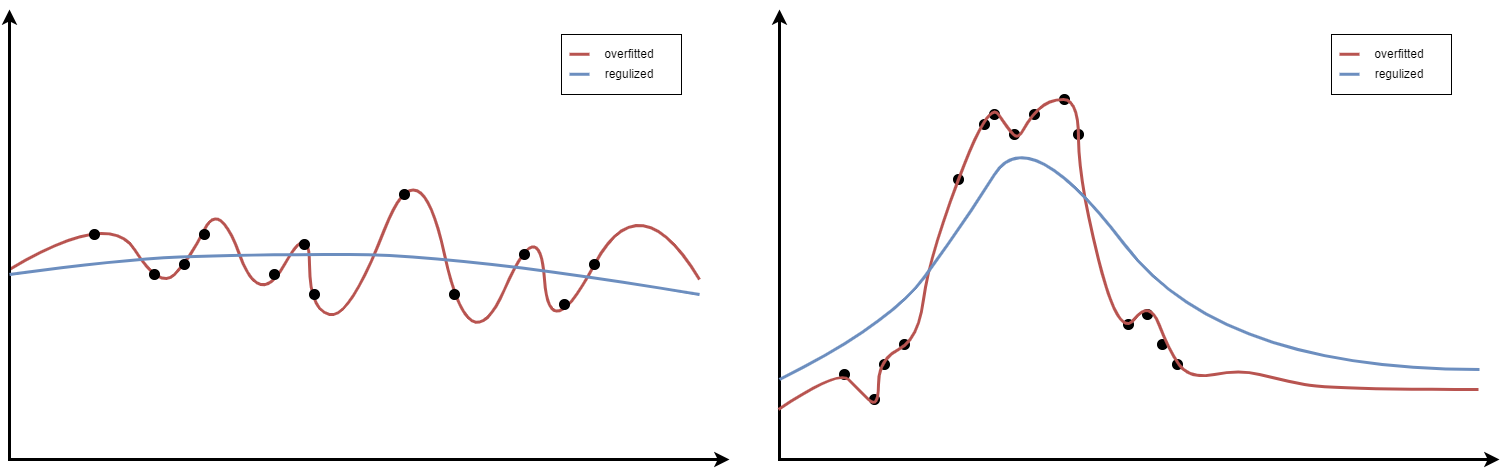
\includegraphics[width= 1\linewidth]{Abschlussarbeit_2021/LaTeX/images/good_baad_to_overfitt.drawio (2).png}
\caption{On the left side, the highly regulated function is to be preferred. On the right side, the perfectly interpolating function performs better. It is also often a question of how much regularization is beneficial}
\end{figure}
%%%
\\
Furthermore the second question that must then be asked is: Can we always reach this said point? We also observed in Chapter 2 that as the size of the data set increases, the underparameterized regime becomes larger and larger and the interpolation threshold shifts further and further to the right (see figure \ref{fig:sample_size_double_descent}). Thus, significantly more variables are needed to memorize larger and larger data sets. Of course, this also shifts the point in the overparameterized regime, from which a better performance is achieved. If we follow the observations from Chapter \ref{experimental_part}, we find that for the MNIST data set, the interpolation threshold, given by the amount of neurons in the hidden layer, can be roughly represented as,
$$
H \leq \frac{n}{1000} 
$$
Where  $n$ is the amount of Data we train with. However the amount of epochs we train also has an impact on the position of the interpolation threshold. Note, that the amount of weights we train depends on the size of the one hidden layer $H$, the input dimension $d = 28\cdot28$ and the output dimension $K = 10$. Therefore the total amount of weights and biases $W$ in the experiment is given by,
$$
W_{MNIST}(H) = (d+1)\cdot H + (H+1) \cdot K
$$
The article by Makhail Belkin gives for the same experiment the number of weights needed with $n\cdot K$ \cite{belkin}. \\
One can imagine that for a more complex problem with a lot of data, such as an image recognition problem, for example IMAGENET, the number of required parameters must be very high. The current record for the largest model is held by the PTD-3 with 175 billion trainable parameters\cite{Artificial_neural_network}. IMAGENET has 14 million images pread across 20,000 different classes \cite{wikipedia_Machine_learning}. With Belkin's formula, you would need for the interpolation threshold alone,
$$
n \cdot K = 14 \cdot 10^{6} \cdot 2 \cdot 10^{4} = 28 \cdot 10^{10}
$$
So 280 billion parameters would be needed. It would probably be impossible even for PTD-3 to memorize the complete data set, let alone get a good performance in the overparameterized regime. Even if the complete IMAGENET data set is never used, there are still many problems that require an incredible amount of data. It could also be observed in chapter \ref{experimental_part} that with more noise in the data set the double descent risk curve is stretched, which makes the required model size even higher. In this case you would have to rely on a good bias variance trade-off. Often there are even meachanisms in models to avoid memorization of the data set. Through weight decay, it can be ensured that models forget their learned weights over time. So of course they also forget the learned training data. For applications, however, this may be less interesting, since the performance at this point is worse than in the underparameterized range.
\\
\subsection{More data can hurt}
Another effect that can occur in the overparameterized regime is that under certain circumstances more data lead to poorer performance. This sounds contradictory at first. And at least for the classic regime, more data is always better. However, as mentioned above, the interpolation threshold shifts further and further to the right for larger sample sizes.\\
For this reason it can happen that for a certain number of parameters the network, which was trained with fewer samples and is therefore already in the overparameterized regime, performs better than the model, which was trained with more data and is therefore in the underparameterized regime. We try to prove this empirically. For this purpose, we always compare two models with one hidden layer, which contains $1 \leq H \leq 50$ neurons each. Both models are trained with the Adams algorithm. The loss function used is sparce-crossentropy and the hidden layer has a RELU-activation function like in \ref{model equation} described. Both models are trained with a subset of MNIST. The first model receives 3000 samples and the second model receives 10000 samples. \\

%%%%Graphen einfügen
\begin{figure}[!htp]
\centering
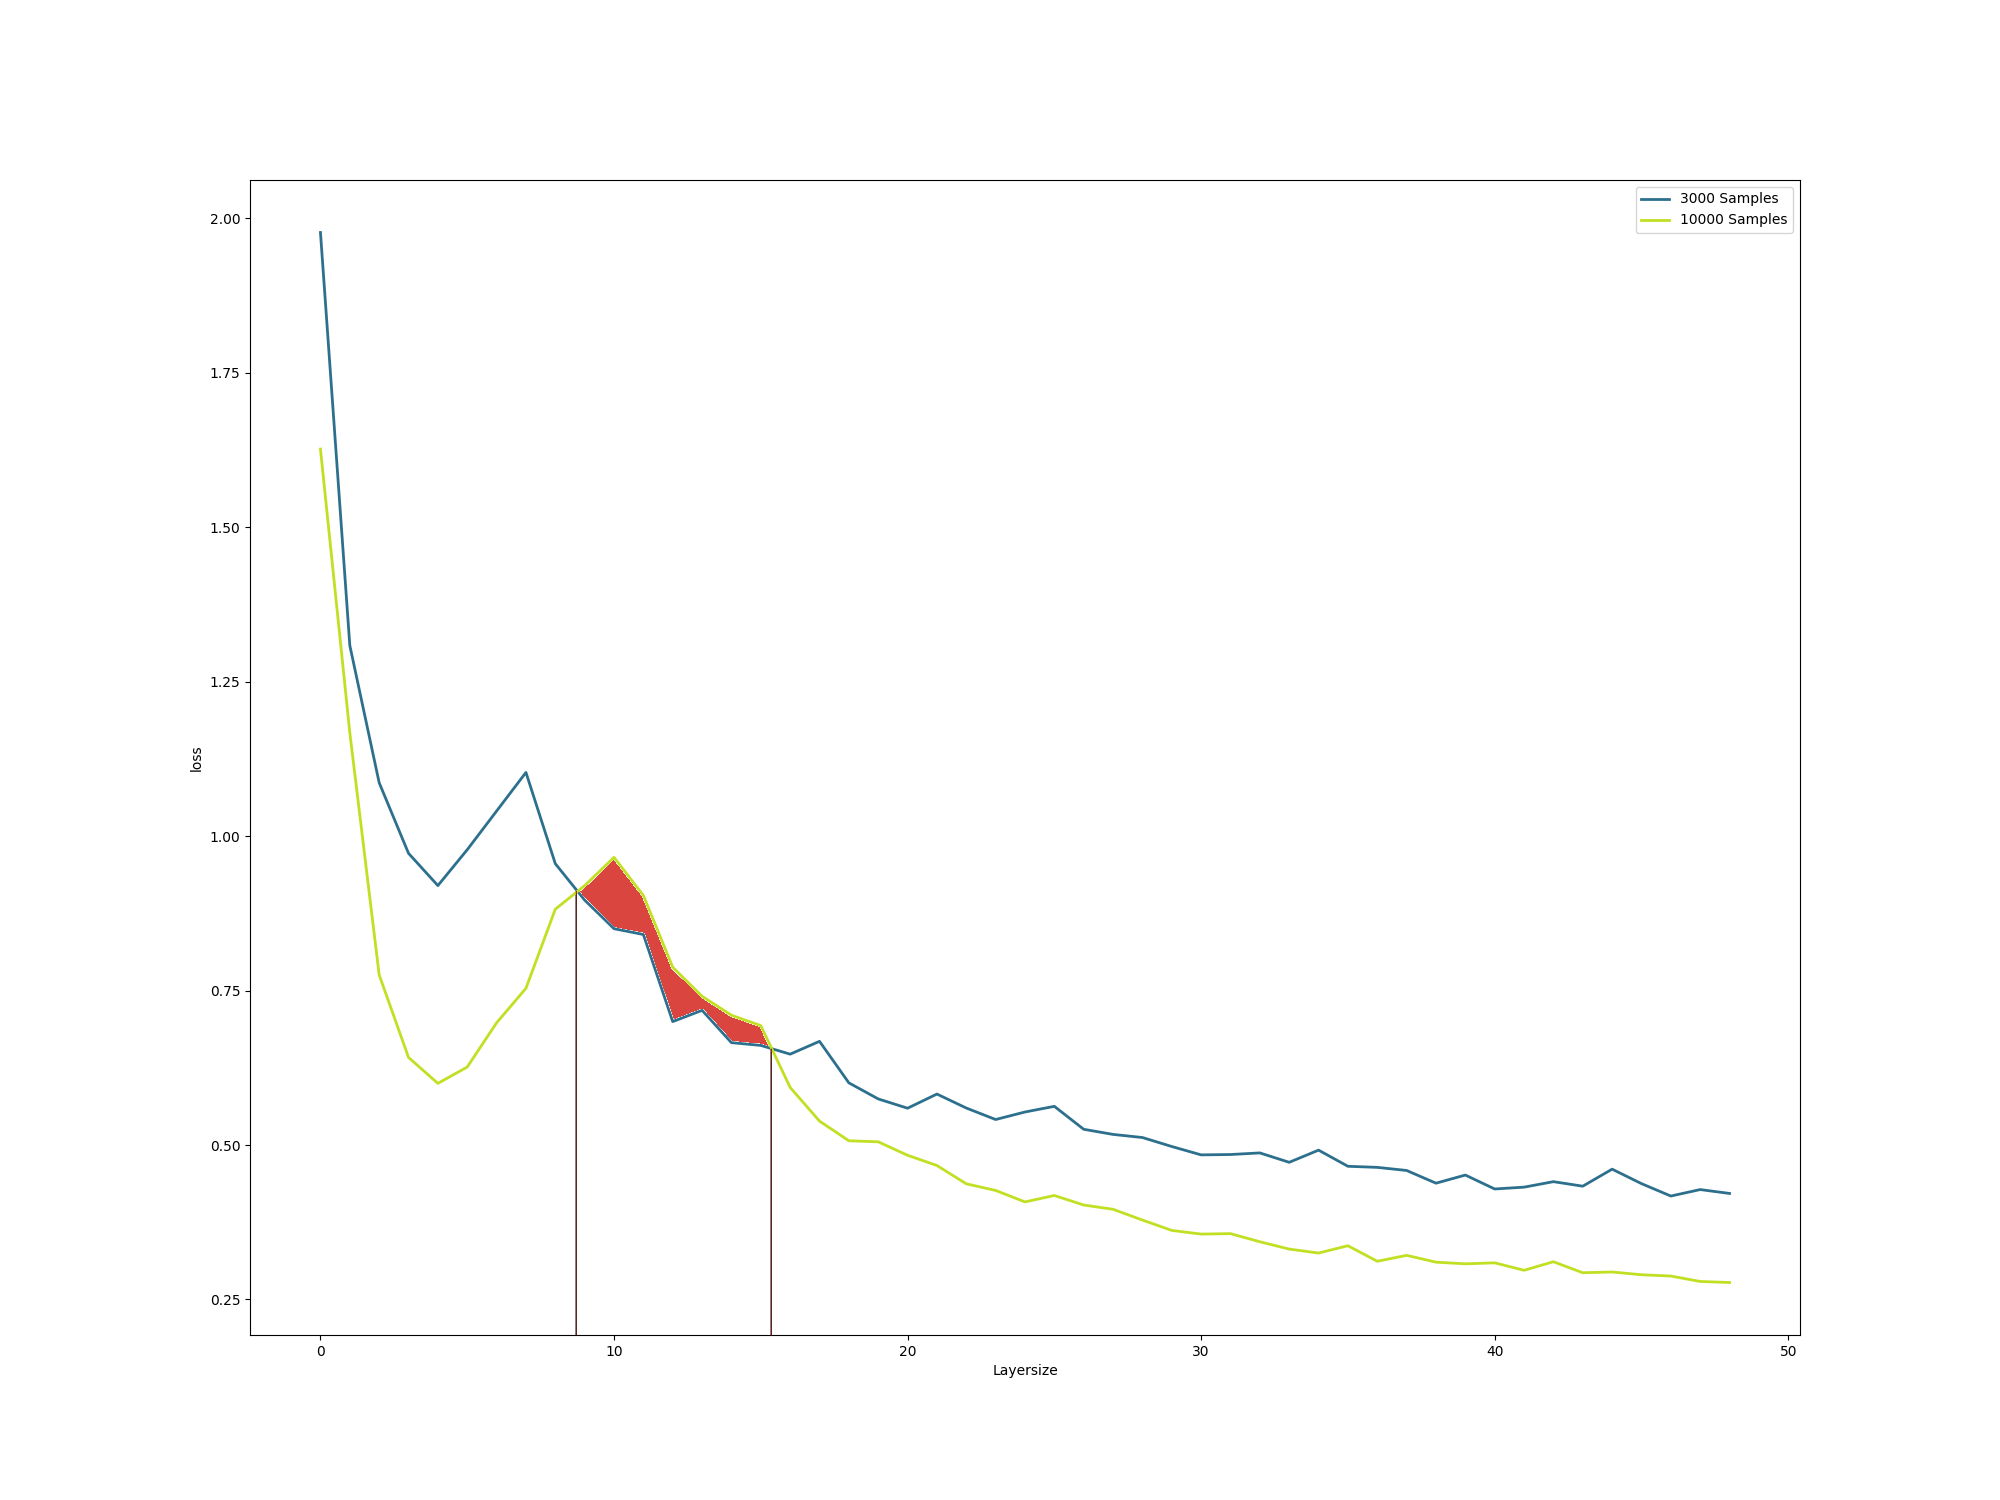
\includegraphics[width= 1\linewidth]{Abschlussarbeit_2021/LaTeX/images/more_is_less.png}
\caption{ Test loss with different sample size. Averaged over 8 runs. The red area indicates the modelsizes, where less data is better}
\label{fig:more_data_hurt}
\end{figure}
%%
%%%describtion ...


The result is shown in figure \ref{less_noise_can_hurt}. With a hidden layer size between $9 \leq H \leq 15$ the model trained with only 3000 samples performs better. 
%%

\subsection{Less noise can hurt}
\label{less_noise_can_hurt}
Another paradoxical phenomenon, which was already observed in chapter \ref{experimental_part}, is that at certain network sizes a higher proportion of noise in the labels can lead to better performance. Therefore, when choosing the model size, it should always be known which noise the data have. Wrong estimation can lead to worse generalization.

%%%
%%%
\begin{figure}[!htp]
\centering
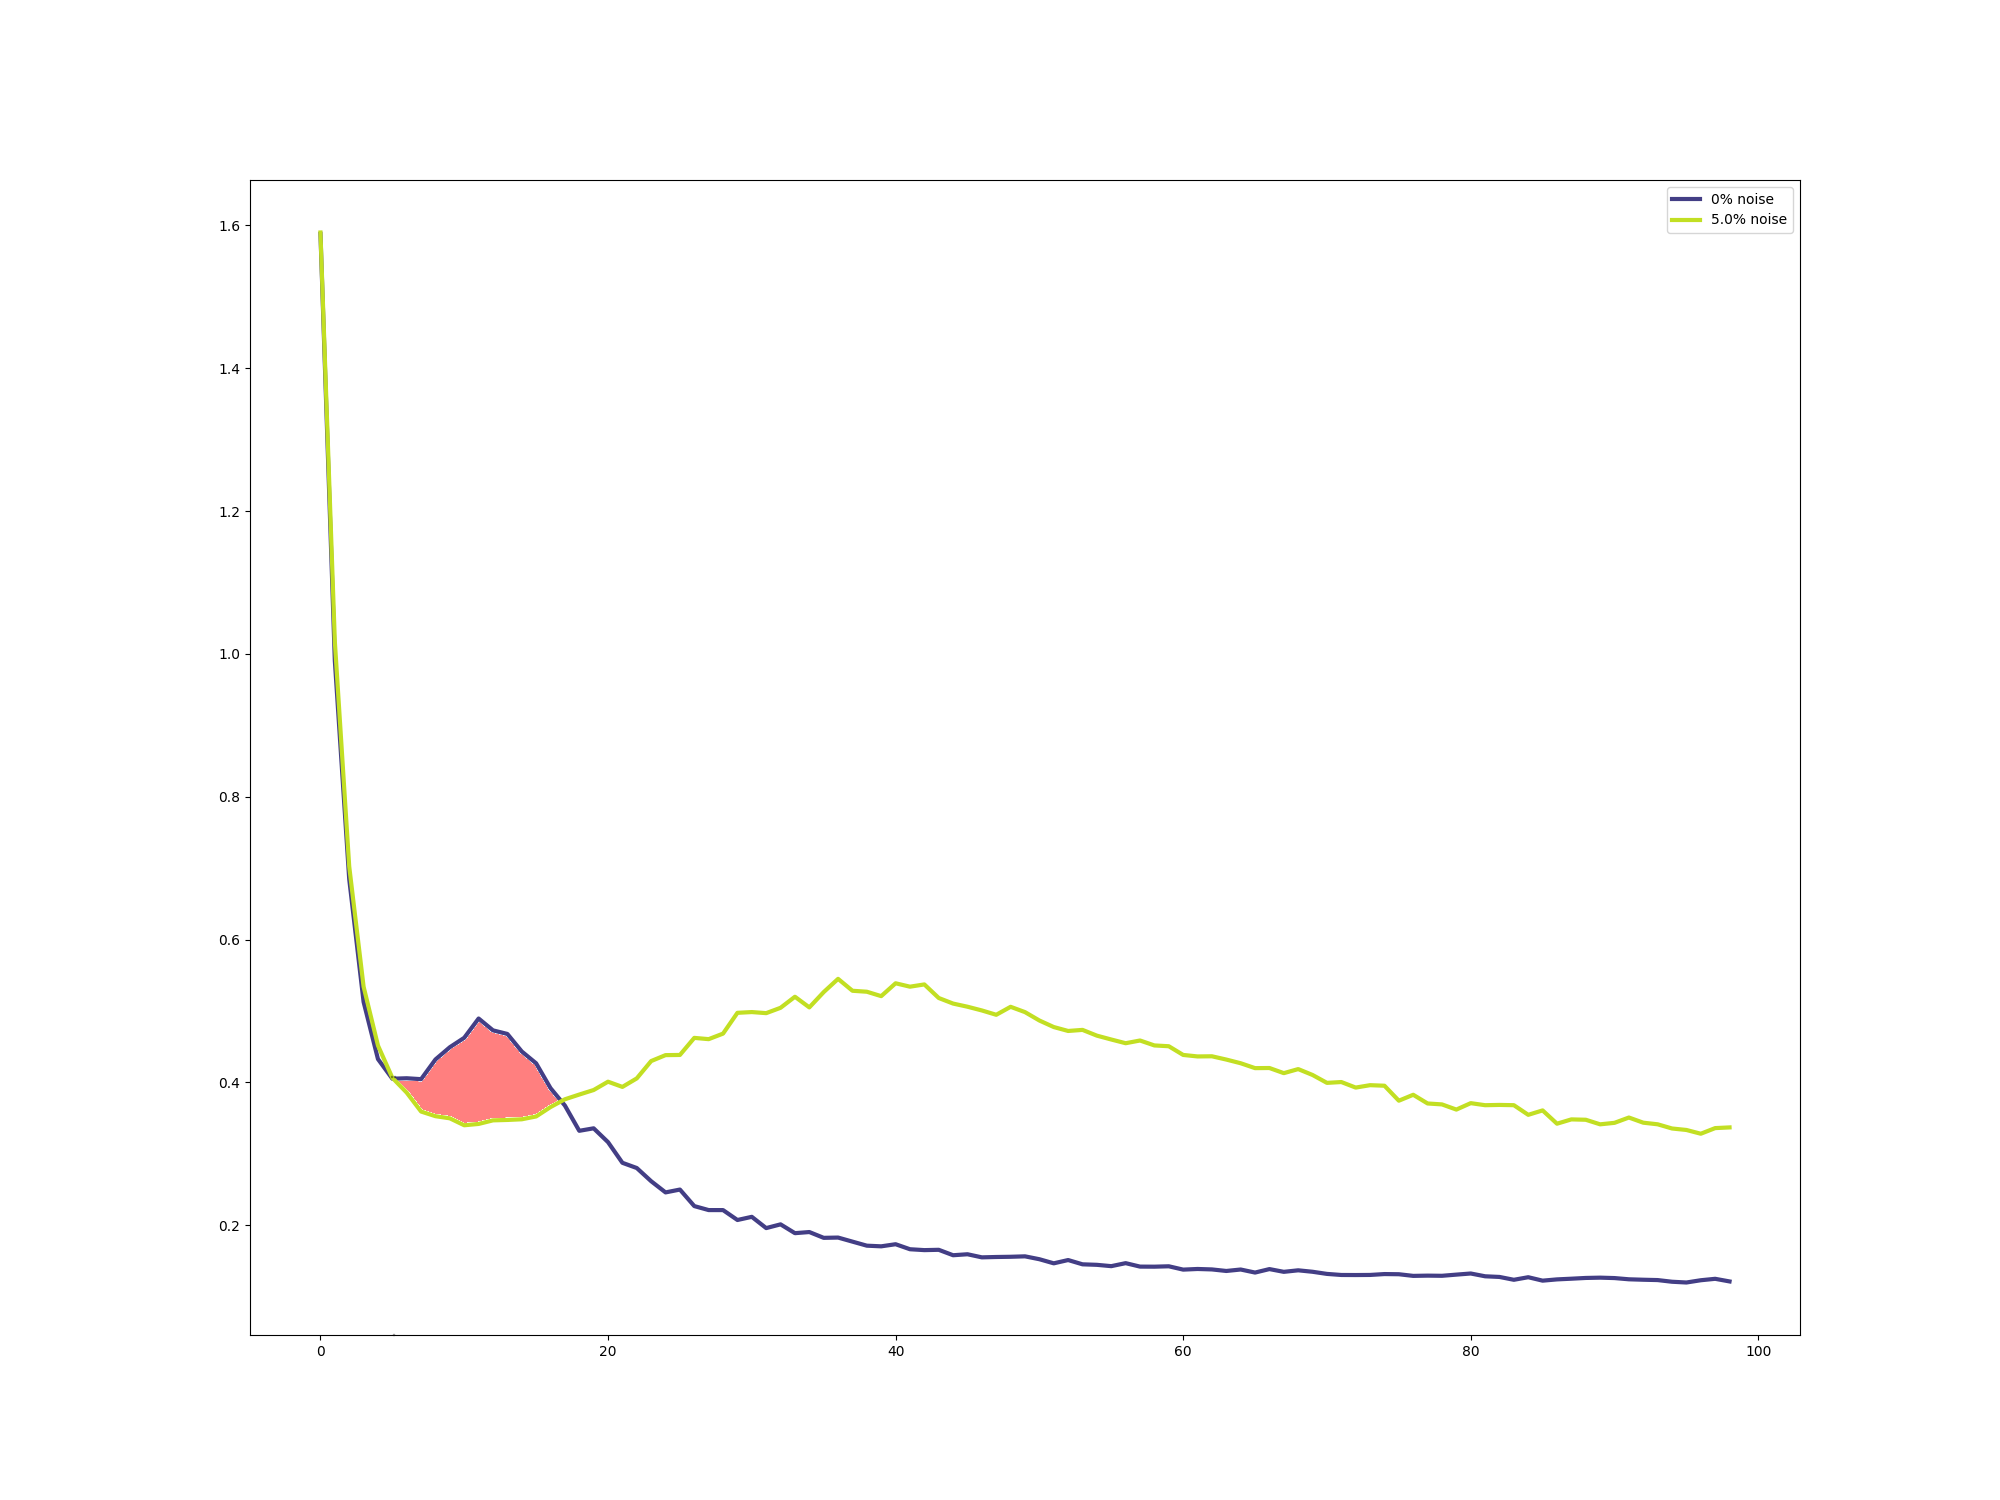
\includegraphics[width= 1\linewidth]{Abschlussarbeit_2021/LaTeX/images/more_noise_hurt.png}
\caption{ Test loss with different label noise. Averaged over 8 runs }
\label{more_noise_can_hurt}
\end{figure}
%%%%

This effect is due to overfitting. Due to the existing noise, it is only possible for networks to interpolate the data set with a high amount of parameters. With a lower amount of parameters the noise in the data set can act as a regularisation term because the Network is far away from interpolating the training data due to the noise. On the other hand, with low noise, overfitting is strong with the same amount of parameters because the interpolation threshold can here be reached much faster.

\subsection{Epoch-weise double descend}
In this thesis, Double Descent was demonstrated only in fully connected neural networks. However double descent can occur all types of neural networks like convolutional-neural-networks and ResNets \cite{Nakkiran_2021_more_data_hurt}. It it is even a phenomenon that occurs in other types of models as well. Double descent is also found in the Random-Forest regression procedure. This was also shown in \cite{belkin}.
However, for the constructed curves we have always changed the number of parameters of the network. Therefore, we can also speak of a parameter-wise double descent. However, there is an additional epoch-wise double descent. This was described for example in \cite{Nakkiran_2021_more_data_hurt}. So there is a similar curve behavior if the model size is fixed but changes the number of epochs. 

\begin{figure}[!htp]
\centering
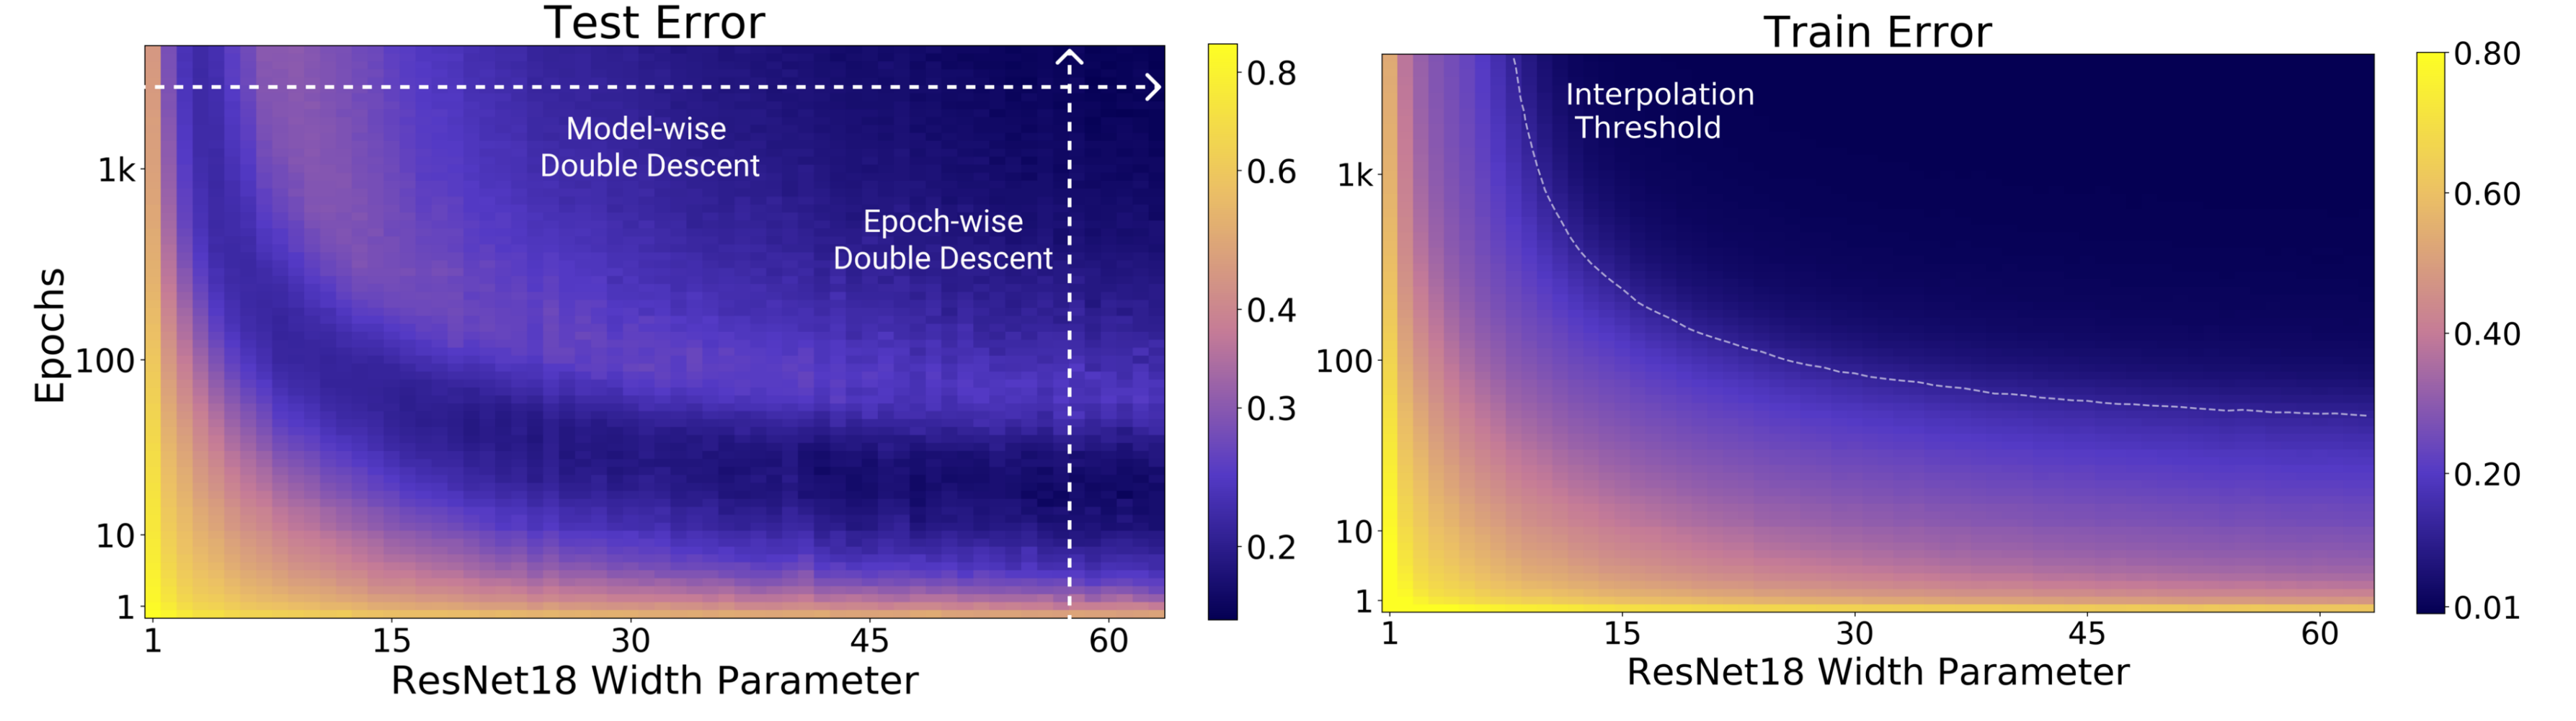
\includegraphics[width= 1\linewidth]{Abschlussarbeit_2021/LaTeX/images/Epochwise.PNG}
\caption{ Figures are taken from \cite{Nakkiran_2021_more_data_hurt}. On the left site the test error can be viewed and on the right side the train error can be seen. the $y$-axis indicates the amount of epochs and the $x$-axes describes the Network size.The convolutional network Resnet18s was trained on CIFAR-10 with 15\% label noise }
\label{fig: epochwise double descent}
\end{figure}

This can also be used under very specific circumstances. However, the epoch-wise double descent probably has less practical application to the training procedure than the parameter-wise variant. It is beyond the scope of this paper to investigate this in more detail. However, the fact that this phenomenon also occurs epoch-wise is highly interesting and is also being extensively researched. It should therefore be mentioned in any case. 







%%%
%%important in this chapter is also, that double descent can occur epochwiese and that double descent %%is even be found in decisiontrees and random forest etc
 
%%
%%larger models are simpler
%%

\newpage

